\documentclass[12pt]{article}
% \usepackage[top=1in,left=1in, right = 1in, footskip=1in]{geometry}
\usepackage[top=1in,footskip=1in]{geometry}

\usepackage{graphicx}
\usepackage{xspace}
%\usepackage{adjustbox}

\usepackage{grffile}

\newcommand{\comment}{\showcomment}
%% \newcommand{\comment}{\nocomment}

\newcommand{\showcomment}[3]{\textcolor{#1}{\textbf{[#2: }\textsl{#3}\textbf{]}}}
\newcommand{\nocomment}[3]{}

\newcommand{\jd}[1]{\comment{cyan}{JD}{#1}}
\newcommand{\swp}[1]{\comment{magenta}{SWP}{#1}}
\newcommand{\bmb}[1]{\comment{blue}{BMB}{#1}}
\newcommand{\djde}[1]{\comment{red}{DJDE}{#1}}

\newcommand{\eref}[1]{Eq.~(\ref{eq:#1})}
\newcommand{\fref}[1]{Fig.~\ref{fig:#1}}
\newcommand{\Fref}[1]{Fig.~\ref{fig:#1}}
\newcommand{\sref}[1]{Sec.~\ref{#1}}
\newcommand{\frange}[2]{Fig.~\ref{fig:#1}--\ref{fig:#2}}
\newcommand{\tref}[1]{Table~\ref{tab:#1}}
\newcommand{\tlab}[1]{\label{tab:#1}}
\newcommand{\seminar}{SE\mbox{$^m$}I\mbox{$^n$}R}

\usepackage{amsthm}
\usepackage{amsmath}
\usepackage{amssymb}
\usepackage{amsfonts}
\usepackage[utf8]{inputenc} % make sure fancy dashes etc. don't get dropped

\usepackage{lineno}
\linenumbers

\usepackage[pdfencoding=auto, psdextra]{hyperref}

\usepackage{natbib}
\bibliographystyle{unsrt}
\date{\today}

\usepackage{xspace}
\newcommand*{\ie}{i.e.\@\xspace}

\usepackage{color}

\newcommand{\Rx}[1]{\ensuremath{{\mathcal R}_{#1}}\xspace} 
\newcommand{\RR}{\ensuremath{{\mathcal R}}\xspace}
\newcommand{\Rres}{\Rx{\mathrm{res}}}
\newcommand{\Rinv}{\Rx{\mathrm{inv}}}
\newcommand{\Rhat}{\ensuremath{{\hat\RR}}}
\newcommand{\Rt}{\ensuremath{{\mathcal R}(t)}\xspace}
\newcommand{\tsub}[2]{#1_{{\textrm{\tiny #2}}}}
\newcommand{\dd}[1]{\ensuremath{\, \mathrm{d}#1}}
\newcommand{\dtau}{\dd{\tau}}
\newcommand{\dx}{\dd{x}}
\newcommand{\dsigma}{\dd{\sigma}}

\newcommand{\rx}[1]{\ensuremath{{r}_{#1}}\xspace} 
\newcommand{\rres}{\rx{\mathrm{res}}}
\newcommand{\rinv}{\rx{\mathrm{inv}}}

\newcommand{\psymp}{\ensuremath{p}} %% primary symptom time
\newcommand{\ssymp}{\ensuremath{s}} %% secondary symptom time
\newcommand{\pinf}{\ensuremath{\alpha_1}} %% primary infection time
\newcommand{\sinf}{\ensuremath{\alpha_2}} %% secondary infection time

\newcommand{\psize}{{\mathcal P}} %% primary cohort size
\newcommand{\ssize}{{\mathcal S}} %% secondary cohort size

\newcommand{\gtime}{\tau_{\rm g}} %% generation interval
\newcommand{\gdist}{g} %% generation-interval distribution
\newcommand{\idist}{\ell} %% incubation-period distribution

\newcommand{\total}{{\mathcal T}} %% total number of serial intervals

\usepackage{lettrine}

\newcommand{\dropcapfont}{\fontfamily{lmss}\bfseries\fontsize{26pt}{28pt}\selectfont}
\newcommand{\dropcap}[1]{\lettrine[lines=2,lraise=0.05,findent=0.1em, nindent=0em]{{\dropcapfont{#1}}}{}}

\begin{document}

\begin{flushleft}{
	\Large
	\textbf\newline{
		Intermediate levels of symptomaticity can lead to the worst population-level outcomes
	}
}
\newline
\\
Joshua Weitz\textsuperscript{1,2,3},
Sang Woo Park\textsuperscript{4},
Jonathan Dushoff\textsuperscript{5,6,7}
\\
\bigskip
\textbf{1} School of Biological Sciences, Georgia Institute of Technology, Atlanta, GA, USA
\\
\textbf{2} School of Physics, Georgia Institute of Technology, Atlanta, GA, USA
\\
\textbf{3} Institut de Biologie, \'{E}cole Normale Sup\'{e}rieure, Paris, France
\\
\textbf{4} Department of Ecology and Evolutionary Biology, Princeton University, Princeton, NJ, USA
\\
\textbf{5} Department of Biology, McMaster University, Hamilton, ON, Canada
\\
\textbf{6} Department of Mathematics and Statistics, McMaster University, Hamilton, ON, Canada
\\
\textbf{7} M.\,G.\,DeGroote Institute for Infectious Disease Research, McMaster University, Hamilton, ON, Canada
\\
\bigskip

\bigskip
\end{flushleft}

SARS-CoV-2 has had devastating effects at the population level.
However, many individuals have mild cases, making it harder to estimate the magnitude of spread and fatality rate. 
The ratio of fatalities to documented cases (the case-fatality rate, CFR) is typically between 1\%--4\%, varying across population because of testing patterns, treatment practice, case definitions, and other factors \%--4\% \citep{rajgor2020many,VERITY2020669,yang2020early}.
But many infections are never documented;
the ratio of fatalities to total infections (the infection fatality rate, IFR) has been estimated to be closer to 0.5\%--1\% for demographics similar to that of the United States \citep{levin2020assessing}. 
This means that more than 99\% of individuals infected with COVID-19 will survive. 
Moreover, at least half of the infections are sufficiently mild that they could be classified as subclinical or even asymptomatic. 

Individuals infected asymptomatically with SARS-CoV-2 can still transmit to others. 
This means that the presence of asymptomatic infections has countervailing effects at the population level. 
On one hand, an asymptomatic infection means that the individual infected avoids hospitalization and fatality. 
On the other hand, asymptomatic infections are less likely to be detected \citep{fraser2004factors}, and may therefore be more likely to infect others, since precautions are less likely to be taken.
This means that the prevalence of asymptomatic infections can paradoxically make population-level outcomes worse than if SARS-CoV-2 was more dangerous at the individual level.

To explore this idea, we propose a simple epidemic model,
in which infected individuals can be asymptomatically or symptomatically infected, with probabilities $p$ and $1-p$, respectively (\fref{base}).  
Asymptomatically infected individuals always recover, whereas a fraction $f$ of symptomatically infected individuals die.
Asymptomatically and symptomatically infected individuals can also have different infection characteristics, including their transmission rates ($\beta_a$ and $\beta_s$) and recovery rates ($\gamma_a$ and $\gamma_s$).
Our key assumption is that symptomatically infected individuals take precautions (e.g., reducing contacts or mask-wearing) and therefore reduce their transmission rate by a fraction $\delta$;
we note that the parameter $\delta$ may also capture intervention measures that target symptomatically infected individuals, such as symptom-based isolation. 
For our main simulations, we assume lower transmission rates for asymptomatically infected individuals ($\beta_a = 0.75 \beta_s$) and equal recovery rates ($\gamma_a = \gamma_s$).
We assume that asymptomatic individuals do not die, and evaluate the effects on population-level mortality of changing the asymptomatic proportion $p$ while holding the fatality rate for \emph{symptomatic} cases, $f$, constant (the IFR $(1-p)f$ thus decreases as $p$ increases).
\jd{It's probably friendlier to talk mostly about \RR, we can then mention $\gamma$ only briefly.}

\begin{figure}[!ht]
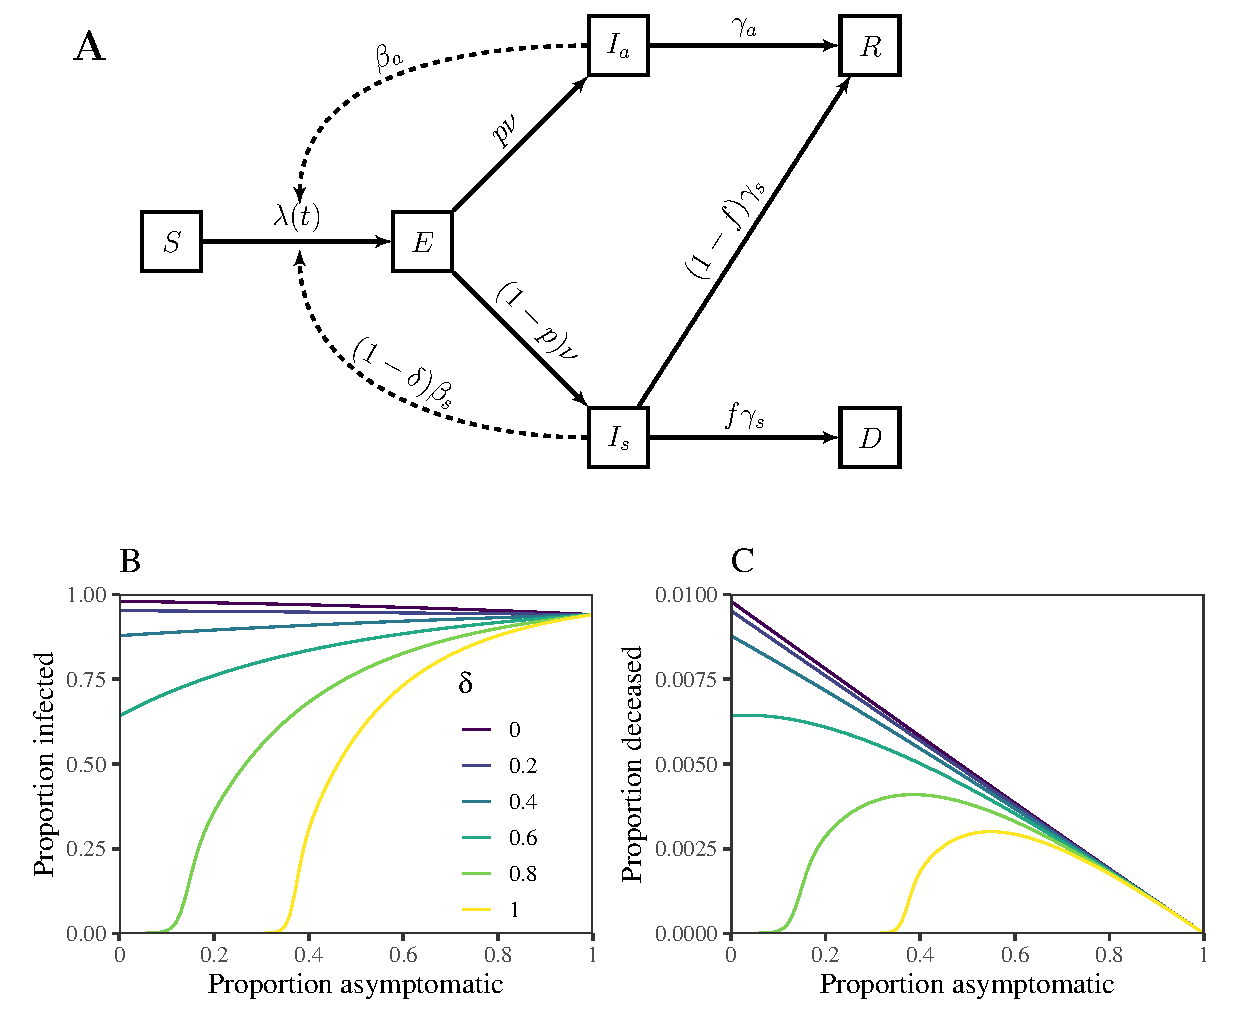
\includegraphics[width=\textwidth]{diagram_base.pdf}
\caption{
\textbf{Schematic diagram and simulations of a model with asymptomatic transmission and symptom-responsive transmission reduction.}
(Left) $S$ represents susceptible individuals; $E$ represents exposed individuals; $I_a$ represents asymptomatically infected individuals; $I_s$ represents symptomatically infected individuals; $R$ represents recovered individuals; and $D$ represents deceased individuals. See Methods for model details.
(Middle) Total infections as a function of the proportion of asymptomatic infections $p$ across a wide range scenarios for $\delta$.
(Right) Total deaths as a function of the proportion of asymptomatic infections $p$ across a wide range scenarios for $\delta$.
We simulate the model for 365 days, assuming $\beta_s = 0.8/\mathrm{day}$, $\beta_a = 0.75 \beta_s$, $\mu=0.5/\mathrm{day}$, $\gamma_s=\gamma_a=0.2/\mathrm{day}$, and $f=0.01$.
We assume that $10^{-4}$ proportion of individuals are initially infected.
}
\label{fig:base}
\end{figure}

\fref{base} shows simulated epidemic outcomes using parameters similar to those of the originating strain of SARS-CoV-2, without any mitigation other than that individuals who are symptomatic reduce their transmission rate by $\delta$. 
In the absence of the behavioral effect ($\delta=0$), the final size decreases with the asymptomatic proportion $p$ because more symptomatic infections leads to a higher basic reproduction number:
\begin{equation}
\RR_0 = (1-p) (1-\delta) \RR_s + p \RR_a,
\end{equation}
where $\RR_s = \beta_s/\gamma_s$ and $\RR_a = \beta_a/\gamma_a$ represent the reproduction numbers of asymptomatic and symptomatic individuals.
This relationship changes as $\delta$ increases.
In particular, when $\delta > 1-\RR_a/\RR_s$ (in our case, $\delta > 0.25)$, the basic reproduction number (and thus epidemic size) increases with $p$ because the effective symptomatic transmission rate (including behavioral response) is less than that the asymptomatic rate.
For $\delta$ in this range, we can find a critical level of asymptomatic proportion, $p_c$:
\begin{equation}
    p_c = \frac{1 - (1-\delta) \RR_s}{\RR_a - (1-\delta) \RR_s}
\end{equation}
such that $p>p_c$ is required for an outbreak. 
\jd{ff.~s.~seems unnecessary:} In the limit that $\delta=1$ (i.e., when symptomatically individuals does not transmit at all), then $p_c=1/\RR_a$.

When behavioral protection is high, the effect of asymptomatic proportion on fatalities shows countervailing effects of individual-level protection and population-level risk.
For high values of $\delta$, the peak fatality occurs at intermediate levels of asymptomatic spread:
although less individuals die per infection for higher values of $p$, the increase in total infections also leads to an increase in total fatalities.
In contrast, when $\delta$ is small enough that $\RR_s\geq\RR_a$, then total fatalities decrease with $p$ because the IFR ($(1-p)f$) decreases.

High values of $\delta$ required for the nonlinear effects of asymptomaticity on deaths may seem unrealistic---in practice, $\delta$ cannot be greater than the amount of post-symptomatic transmission.
While several studies have estimated the proportion of pre-symptomatic transmission to be around 30\%--60\% for the SARS-CoV-2 wildtype strain, many of them were likely subject to intervention and behavioral effects already as they were conducted after SARS-CoV-2 awareness became widespread \citep{he2020temporal}.
Instead, \cite{sender2021unmitigated} recently showed that the proportion of pre-symptomatic transmission can be as low as 20\% (95\%CI: 6\%--32\%) in the absence of intervention measures;
while this study provides indirect support for the feasibility of high $\delta$ values, it is still uncertain whether similar effects can be found in more realistic settings.
\jd{We need to be a bit more nuanced here: we get the low value by focusing on just a couple of weeks, so we're sort of suggesting a counter-factual where nobody notices COVID for a long time.}

We therefore consider two additional of mathematical models with increasing complexities to answer a more general question:
does intermediate amount of subclinical (including both asymptomatic and presymptomatic) transmission lead to peak fatalities?
First, we analyze a model with presymptomatic transmission alone (Supplementary Figure S1).
When the reproduction number is fixed, increasing the proportion of presymptomatic transmission $\theta$ causes larger outbreaks, and therefore more deaths, in the presence of symptom-responsive transmission reduction ($\delta > 0$).
However, standard compartmental models implicitly assume that the fatality rate $f$ is independent of the amount of presymptomatic transmission---in the extreme case where all transmission happens presymptomatically, infected individuals no longer shed infectious virus after symptom onset, meaning that they should be less likely to die from infection.
\jd{We need a bit more detail here. I have no idea what proportion of COVID deaths are post-viral. Maybe I'm COVID-ignorant, but I want more info: many flu deaths are post-viral, and it's not super-clear how much of a role viral replication (or escape from deep lungs?) plays in fatality.}
We therefore assume a tradeoff between the amount of presymptomatic transmission $\theta$ and the fatality rate $f$ that follows a power law: $f(\theta) = f_0 (1-\theta^a)$, which monotonically decreases from $f_0$ to 0.
In the simple case where the fatality rate decreases linearly with $\theta$, the relationship between the amount of presymptomatic transmission $\theta$ and total fatalities is equivalent to that between the amount of asymptomatic transmission and total fatalities in the original model (\fref{base}).
As we increase the exponent $a$, we obtain a more realistic tradeoff curve such that fatality rate $f$ remains roughly constant for low to intermediate values of $\theta$ and suddenly decreases to $0$ as $\theta$ approaches 1;
in these cases, peak fatalities occur at intermediate levels of presymptomatic transmission for even lower values of $\delta=0.6$, which now represents reduction in transmission after symptom onset.

We then extend our model to consider the effects of generalized \textit{subclinical} transmission, which includes both presymptomatic and asymptomatic transmission (Supplementary Figure S2).
In particular, we fix the reproduction number of symptomatic individuals and calculate the proportion of deceased individuals for given values of proportion of total subclinical transmission and proportion of subclinical transmission that is caused by presymptomatic transmission.
This model generalizes two earlier models:
when all subclinical transmission is caused by asymptomatic transmission, we have the first model (\fref{base});
and when all subclinical transmission is caused by presymptomatic transmission, we have the second model (Supplementary Figure S1).
We find a wide variety of scenarios for which peak fatalities occur at intermediate levels of subclinical transmission in the presence of moderate to strong behavioral effect, $\delta > 0.6$ (Supplementary Figure S2);
this pattern is robust even to the absence of a tradeoff between the amount of presymptomatic transmission and the fatality rate.
One exception is the case discussed earlier in which all subclinical transmission is caused by presymptomatic transmission.
Hereafter, we focus on asymptomatic infections for simplicity, but our conclusions have implications for the more general case of subclinical transmission.

We now apply our framework to understand the impact of immunity on the severity of the disease by dividing the population into two groups: immunologically naive and protected.
The dynamics of immunologically naive individuals are equivalent to our original model (\fref{base}).
The dynamics of protected individuals include three additional parameters, which characterize the amount of protection against infection $\epsilon_i$, symptoms $\epsilon_s$, and deaths $\epsilon_d$ (\fref{immune}).
For simplicity, we assume that the population is exactly split in half (50\% naive and 50\% protected) and mixes homogeneously; we do not consider the separate effect of immunity on transmission (beyond the effect on infection).
We assume a relatively strong behavioral effect $\delta=0.8$ for illustration.

\begin{figure}[!ht]
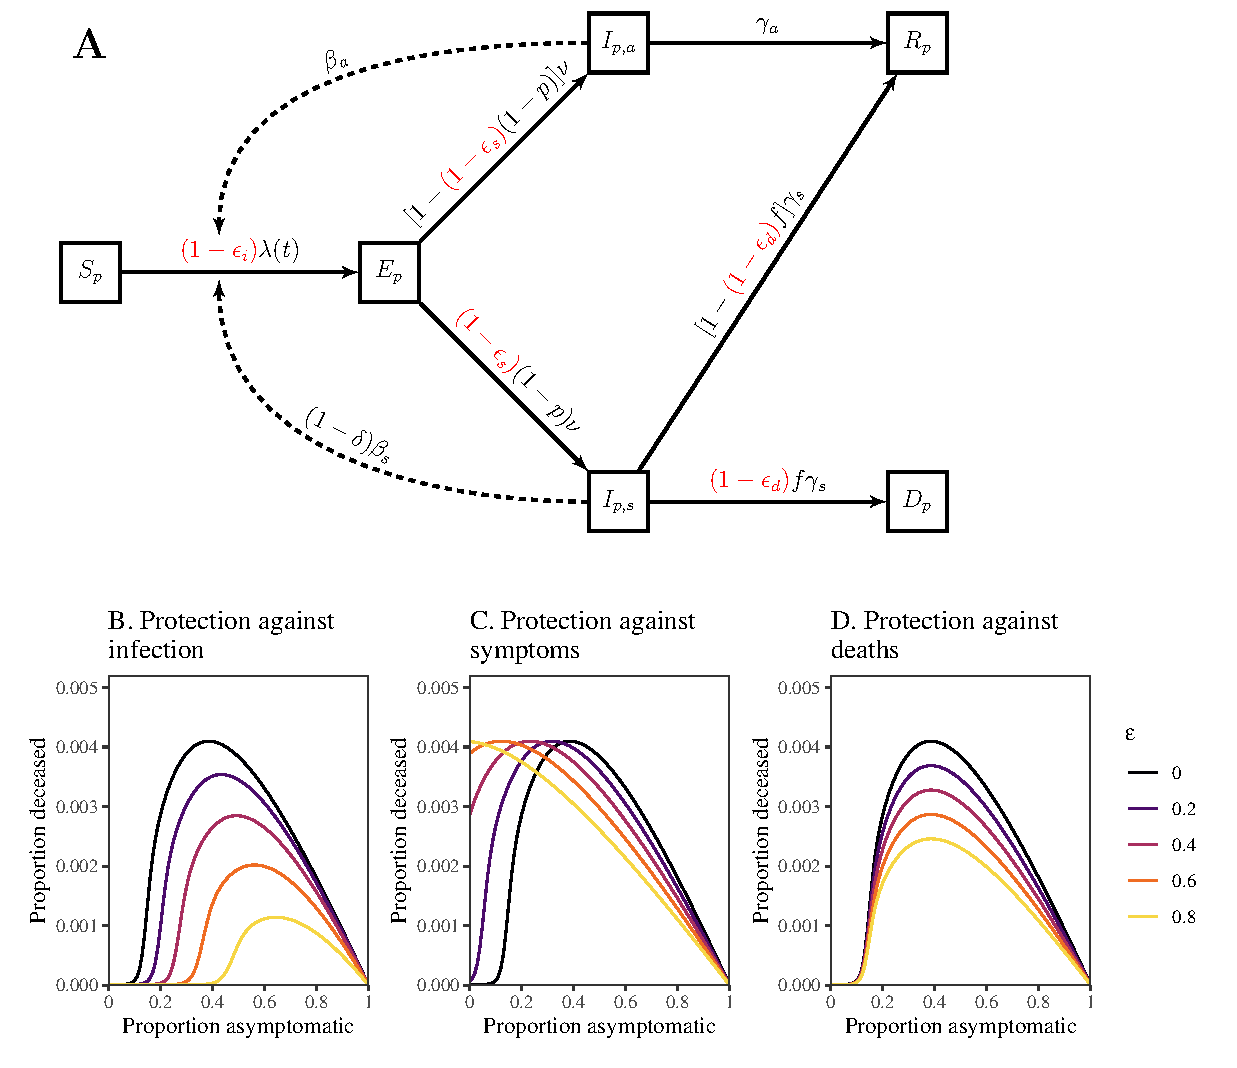
\includegraphics[width=\textwidth]{diagram_immune.pdf}
\caption{
\textbf{Schematic diagram and simulations of a model with symptom-responsive transmission reduction and immunity.}
(Top) The subscript $p$ represents protected individuals. 
Immunity may provide protection against infection, symptoms, or deaths.
The dynamics of immunologically naive individuals are described in (\fref{base}).
(Bottom) Total deaths as a function of the proportion of asymptomatic infections $p$ across a wide range scenarios for protection against infection $\epsilon_i$, symptoms $\epsilon_s$, and deaths $\epsilon_d$.
We simulate the model for 365 days, assuming $\beta_s = 4/5/\mathrm{day}$, $\beta_a = 0.75 \beta_s$, $\mu=1/2/\mathrm{day}$, $\gamma_s=\gamma_a=1/5/\mathrm{day}$, $f=0.01$, and $\delta=0.8$.
We assume that $10^{-4}$ proportion of individuals are initially infected.
}
\label{fig:immune}
\end{figure}

The impact of protection against infection $\epsilon_i$ is analogous to changing $\RR_0$ in the original model: as immunity provides stronger protection against infection (higher $\epsilon_i$), the number of deaths decreases and a higher asymptomatic fraction $p$ is required for the infection to spread (\fref{immune}A).
We note that protection against infection scales the fatality curve nonlinearly, reflecting the nonlinear relationship between $\RR_0$ and the final size.
The impact of protection against symptoms $\epsilon_s$ is exactly equivalent to changing fraction asymptomatic $p$ for the protected population:
the fatality curves move left as we increase the degree of protection $\epsilon_s$ (\fref{immune}B).
Therefore, for low values of $p$, protection against symptoms can inadvertently increase the total number of fatalities at the population level by increasing the proportion (and number) of asymptomatically infected individuals, who can readily transmit infections to other individuals.
This also means that the critical level of asymptomatic proportion decreases, allowing more dangerous infections (with lower $p$) to invade, which would not have been able to spread in an otherwise immunologically naive population.
Protection against deaths $\epsilon_d$ directly modulates the fatality rate for symptomatic cases and therefore linearly scales the fatality curves (\fref{immune}C).

\begin{figure}[!ht]
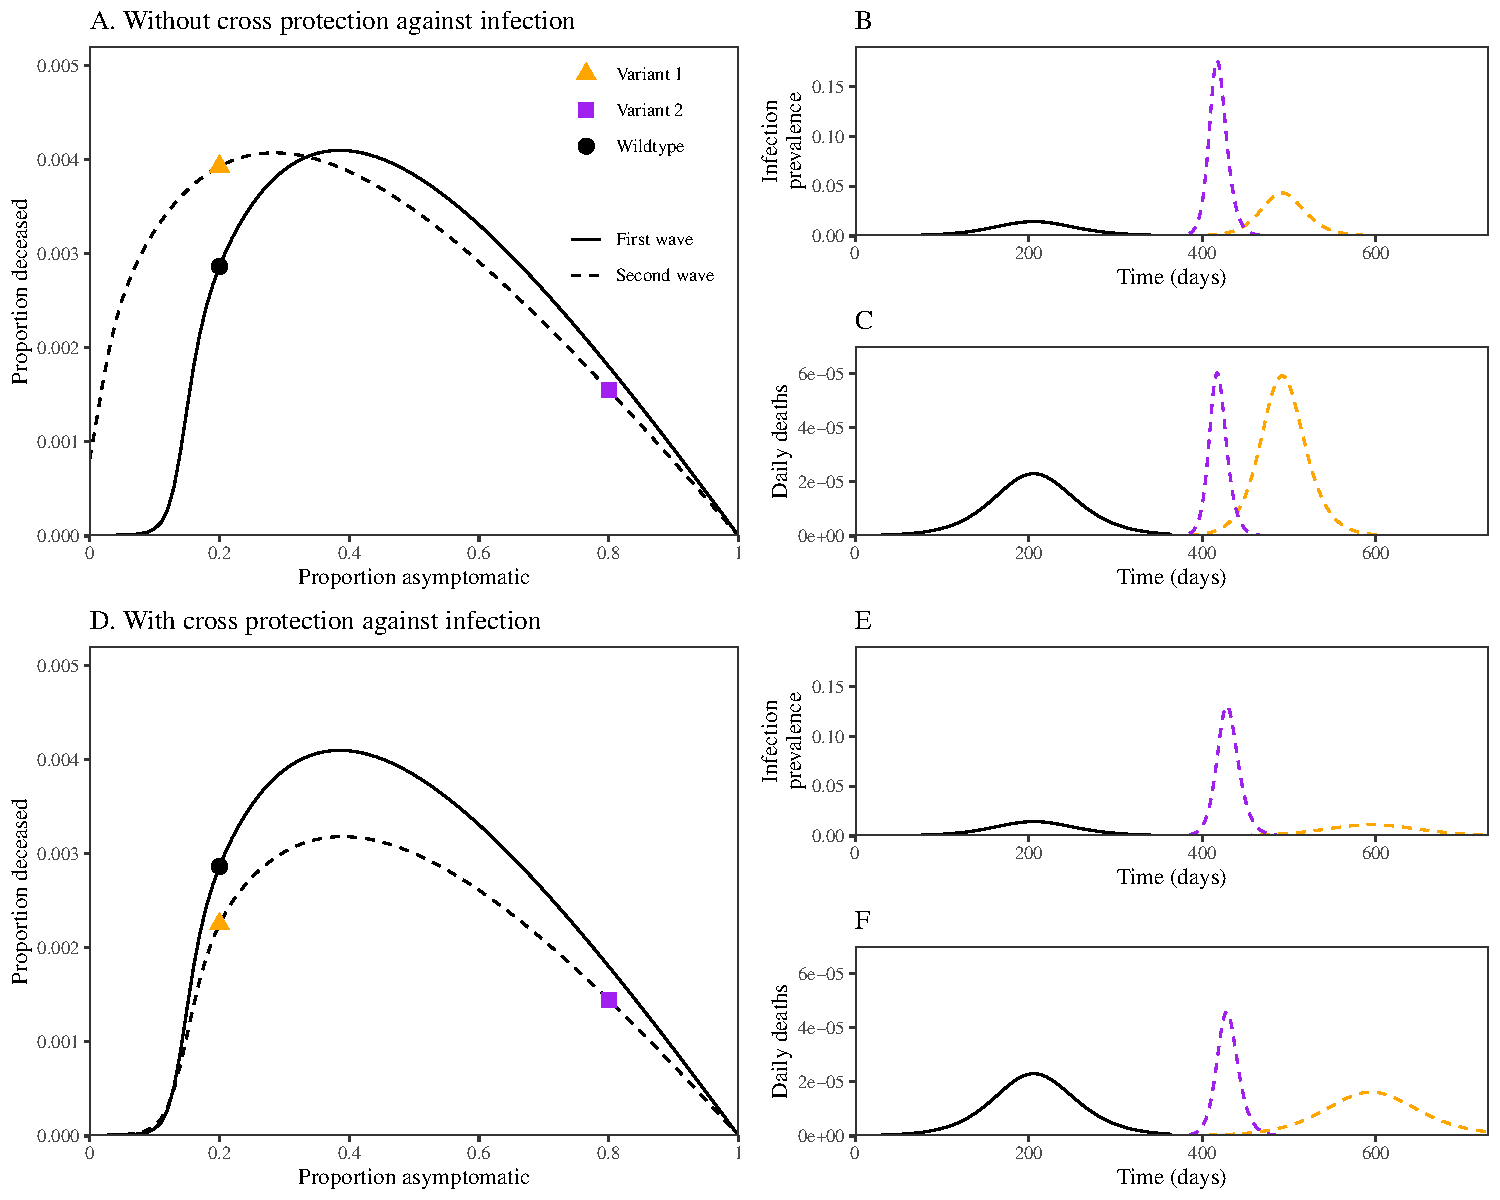
\includegraphics[width=\textwidth]{figure_variant.ggp.pdf}
\caption{
\textbf{Dynamics of invading variants under symptom-responsive transmission reduction and immunity.}
(A, D) Asymptomaticity--fatality curves for the first (solid lines) and second waves (dashed lines).
Points represent specific scenarios we assume for the first and second waves.
Fatality curves for the first wave are calculated by simulating an epidemic for 1 year using same parameters as \fref{base} and $\delta=0.8$.
Fatality curves for the second wave are calculated by first simulating the first wave assuming $p=0.2$ (wildtype) for 1 year to calculate the proportion immune and then simulating the extended model presented in \fref{immune}.
(B, E) Dynamics of infection prevalence for the wildtype variant (black, solid line) and two possible invading variants (colored, dashed line).
(C, F) Dynamics of daily deaths for the wildtype variant (black, solid line) and two possible invading variants (colored, dashed line).
}
\label{fig:variant}
\end{figure}

Finally, we use our framework to understand the impact of behavioral effects on invading variants (\fref{variant}).
In doing so, we first simulate the dynamics of a wildtype variant for 1 year using our base model (\fref{base}).
We then simulate a new variant invading a partially immune population using our extended model (\fref{immune}), where the immunity is solely derived from natural infections caused by the wildtype variant.
We consider two types of variants (which are simulated separately): one with the same severity $p$ (variant 1, orange) and a milder one with higher $p$ (variant 2, purple).

First, we consider a scenario in which immunity only provides protection against symptoms, $\epsilon_s = 0.4$ (\fref{variant}A--C).
In this case, protection against symptoms allows new variants to spread faster, resulting in larger outbreaks (\fref{variant}B).
Although, a milder (purple) variant exhibits a faster epidemic growth rate and reaches a higher peak (\fref{variant}B), it reaches similar peak fatality as the more severe (orange) variant (\fref{variant}C).
The asymptomaticity--fatality curve provides additional insight (\fref{variant}A): even though a milder, invading variant (purple square) gives higher peak fatality than the original, wildtype variant (black circle), it leads to lower fatalities overall because deaths are concentrated over a shorter period of time.
In general, invading variants with similar asymptomaticity $p$ will spread better and result in worse population-level outcomes if immunity (either from vaccination or natural infection) provides protection against symptoms, given that asymptomatically infected individuals can transmit better than symptomatically infected individuals (due to either behavioral and intervention effects).

Next, we consider a more realistic scenario in which immunity provides protection against symptoms, $\epsilon_s = 0.4$, and infection, $\epsilon_i = 0.4$ (\fref{variant}D--F).
In this case, cross protection against infection has a disproportionately larger effect on the more severe (orange) variant, causing its peak infection prevalence (\fref{variant}E) and fatality (\fref{variant}F) to be lower than that of the original, wildtype variant.
Across a wide range of asymptomatic proportion $p$, we find that this immunity profile is sufficient to prevent worse outcomes at the population level.

In summary, using a simplified model we have shown that asymptomatic infections can represent a double-edge sword insofar as they represent a better outcome for some individuals but a mechanism for onwards transmission that leads to a worse outcome for the population as a whole.
Extending our framework further shows that the immunity profile plays a critical role in determining the dynamics of future variants:
while protection against symptoms prevent diseases at the individual level, it can inadvertently lead to more infections, and potentially deaths, at the population level.
For example, milder variants can result in even faster epidemic growth rates and larger outbreaks, even though it can lead to less fatalities if the variant is sufficiently mild.

Our simulations of invading variants resemble the dynamics of the SARS-CoV-2 Omicron variant.
Despite moderate levels of vaccine effectiveness against symptomatic and severe cases caused by the Omicron variant, especially after booster shots \citep{andres2022omicron}, both vaccine- and infection-derived immunity has provided limited protection against infections \citep{pearson2021omicron}.
Its immune evasive property allowed the Omicron variant to cause more infections in South Africa than previous variants \citep{sun2022omicron};
therefore, even though the Omicron variant has been estimated to be milder \citep{MENNI20221618,ulloa2022estimates}, the number of hospitalizations and deaths caused by the Omicron variant have remained high \citep{Iacobuccio254,faust2022omicron,sigal2022estimating}.

There are several limitations to our analysis.
First of all, behavioral and intervention effects must sufficiently high in order for the fatality to peak at intermediate levels of asymptomaticity.
While we are able to generalize our results using more realistic models, incorporating both presymptomatic and asymptomatic transmission, the transmission rate needs to be reduced by at least 60\% after symptom onset for us to see the nonlinear effects of subclinical transmission on population-level outcomes.
\swp{what are some other limitations we should address?}

SARS-CoV-2 has proven hard to control in large part because transmission is often decoupled from symptoms. 
Although mitigation efforts have often prioritized responding to symptoms---including symptom-based testing, fever checks, mask-wearing for infectious individuals---a different approach that strives to reduce the chance of asymptomatic transmission while increasing treatment of symptomatically infected individuals could both reduce infection risk at the source and in the event that individuals are at risk for severe outcomes.
As more variants continue to emerge, updating vaccines to prevent infections, and not just diseases, will be critical to controlling the course of the pandemic.

\pagebreak

\section*{Supplementary Materials}
\setcounter{figure}{0}
\renewcommand{\thefigure}{S\arabic{figure}}

\subsection*{Methods}

\subsubsection*{Models without immunity}

First, we consider a simple, compartmental model with asymptomatic and symptomatic infections in a homogeneously mixing population.
The model dynamics are as follows:
\begin{align}
\dot{S} &= -\beta_a S I_a -(1-\delta) \beta_s S I_s \\
\dot{E} &= \beta_a S I_a + (1-\delta) \beta_s S I_s - \mu E\\
\dot{I}_a &= p \mu E - \gamma_a I_a\\
\dot{I}_s &= (1-p) \mu E -\gamma_s I_s\\
\dot{R} &= \gamma_a I_a + (1-f) \gamma_s I_s \\
\dot{D} &= f \gamma_s I_s
\end{align}
where the transmission rate $\beta$ and recovery rate $\gamma$ can be potentially differ between asymptomatic and symptomatically infected individuals.  
Here, $\delta$ denotes the reduction in transmissibility due to responsive measures taken by symptomatically infected individuals.
Throughout the paper, we use parameters that are broadly consistent with the dynamics of the originating strain of SARS-CoV-2: $\beta_s = 0.8/\mathrm{day}$, $\beta_a = 0.75 \beta_s$, $1/\mu=2\,\mathrm{days}$, $1/\gamma_s=1/\gamma_a=5\,\mathrm{days}$, and $f=0.01$.

We then consider a model with presymptomatic transmission (and without asymptomatic transmission), where all infected individuals eventually develop symptoms:
\begin{align}
\dot{S} &= -\beta_a S I_a -(1-\delta) \beta_s S I_s \\
\dot{E} &= \beta_a S I_a + (1-\delta) \beta_s S I_s - \mu E\\
\dot{I}_p &= \mu E - \sigma I_p\\
\dot{I}_s &= \sigma I_p -\gamma_s I_s\\
\dot{R} &= (1-f) \gamma_s I_s \\
\dot{D} &= f \gamma_s I_s
\end{align}
For this model, the presymptomatic $\RR_p$ and symptomatic $\RR_s$ reproduction numbers are given by $\RR_p = \beta_p/\sigma$ and $\RR_s=\beta_s/\gamma_s$ in the absence of the behavioral effect; and the basic reproduction number is equal to the sum of the two.
Then, the intrinsic proportion of presymptomatic transmission is given by: 
\begin{equation}
\theta = \frac{\RR_p}{\RR_p + \RR_s}.
\end{equation}
We assume there is a tradeoff between the proportion of presymptomatic transmission and fatality rate: 
\begin{equation}
f(\theta) = f_0 (1-\theta^a),
\end{equation}
where $f_0=0.01$ represents the baseline fatality rate and the exponent $a$ is varied between 1 and 5.
Throughout simulations, we assume $\mathcal R_0 = 4$, $1/\sigma=2\,\mathrm{days}$, and $1/\gamma_s=3\,\mathrm{days}$.
All other parameters are same as before.

Finally, we combine both models to include both presymptomatic and asymptomatic transmission:
\begin{align}
\dot{S} &= -\beta_a S I_a -(1-\delta) \beta_s S I_s \\
\dot{E} &= \beta_a S I_a + (1-\delta) \beta_s S I_s - \mu E\\
\dot{I}_p &= \mu E - \sigma I_p\\
\dot{I}_a &= p \sigma I_p - \gamma_a I_a\\
\dot{I}_s &= (1-p) \sigma I_p -\gamma_s I_s\\
\dot{R} &= \gamma_a I_a + (1-f) \gamma_s I_s \\
\dot{D} &= f \gamma_s I_s
\end{align}
For this model, the reproduction number of individuals who will eventually develop symptoms is equal to: $\RR_p + \RR_s$;
similarly, the reproduction number of individuals who remain asymptomatic is equal to: $\RR_p + \RR_a$.
Since proportion $p$ of all infections is asymptomatic, the basic reproduction number is given by the weighted average of these two reproduction numbers: 
\begin{equation}
\RR_0 = p(\RR_p + \RR_a) + (1-p) (\RR_p + \RR_s) = \RR_p + p \RR_a + (1-p) \RR_s.
\end{equation}
Then, the proportion of subclinical transmission $\phi$ is given by:
\begin{equation}
\phi = \frac{\RR_p + p \RR_a}{\RR_0}.
\end{equation}

For simulations of the combined model, we start by fixing the reproduction number of individuals who will eventually develop symptoms: $\RR_{\textrm{symp}} = \RR_p + \RR_s = 4$. 
Consistent with previous assumptions, we also assume that asymptomatic reproduction number is lower than that of the symptomatic reproduction number: $\RR_a = \rho \RR_s$ where $\rho = 0.75$.
Then, for a given value of the proportion of subclinical transmission $\phi$ and proportion of subclinical transmission caused by the presymptomatic transmission, $\eta = \RR_p/(\RR_p + p \RR_a)$, we can solve for the transmission rate for each compartment $\beta$ and the proportion asymptomatic $p$.
More specifically:
\begin{align}
\RR_p &= \frac{\RR_{\textrm{symp}}}{1 + y}\\
\RR_s &= \RR_{\textrm{symp}} - \RR_p\\
\RR_a &=  \rho \RR_s\\
p &= \left(\frac{1}{\eta} - 1 \right) \frac{\RR_p}{\RR_a},
\end{align}
where $y = (1/\phi - 1)/\eta + (1/\eta - 1)/\rho$.
All other parameters are same as before.

\subsubsection*{Model with immunity}

We then model the spread of infection in a partially immune population.
The model dynamics are as follows:
\begin{align}
\dot{S} &= -\lambda (t) S \\
\dot{E} &= \lambda (t) S - \mu E\\
\dot{I}_a &= p \mu E - \gamma_a I_a\\
\dot{I}_s &= (1-p) \mu E -\gamma_s I_s\\
\dot{R} &= \gamma_a I_a + (1-f) \gamma_s I_s \\
\dot{D} &= f \gamma_s I_s\\
\dot{S}_p &= - (1-\epsilon_i) \lambda (t) S_p \\
\dot{E}_p &= (1-\epsilon_i) \lambda (t) S_p - \mu E_p\\
\dot{I}_{p, a} &= (1 - (1-\epsilon_s) (1-p)) \mu E_p - \gamma_a I_{p,a}\\
\dot{I}_{p, s} &= (1-\epsilon_s) (1-p) \mu E_p -\gamma_s I_{p,s}\\
\dot{R}_p &= \gamma_a I_{p,a} + (1-(1-\epsilon_d) f) \gamma_s I_{p,s} \\
\dot{D}_p &= (1-\epsilon_d) f \gamma_s I_{p,s}
\end{align}
where $\epsilon$ represents the degree of protection against infection, symptoms and death. 
The force of infection $\lambda(t)$ is given by:
\begin{equation}
\lambda(t) = \beta_a (I_a + I_{p,a}) + (1-\delta) \beta_s (I_s + I_{p,s}).
\end{equation}
Here, subscripts $p$ denote individuals who are immune and therefore are protected.

\pagebreak

\section*{Supplementary Figures}

\begin{figure}[!h]
\begin{center}
\includegraphics[width=0.7\textwidth]{diagram_pre.pdf}
\caption{
\textbf{Schematic diagram and simulations of a model with presymptomatic transmission and symptom-responsive transmission reduction.}
(Top) $S$ represents susceptible individuals; $E$ represents exposed individuals; $I_p$ represents presymptomatically infected individuals; $I_s$ represents symptomatically infected individuals; $R$ represents recovered individuals; and $D$ represents deceased individuals. See Methods for model details.
(Bottom) Total deaths as a function of the proportion of presymptomatic transmission $\theta$ across a wide range scenarios for $\delta$ and a tradeoff between the proportion of presymptomatic infections $\theta$ and fatality rates $f$.
}
\end{center}
\end{figure}

\pagebreak

\begin{figure}[!ht]
\begin{center}
\includegraphics[width=0.7\textwidth]{diagram_sub.pdf}
\caption{
\textbf{Schematic diagram and simulations of a model with presymptomatic and asymptomatic transmission and symptom-responsive transmission reduction.}
(Top) $S$ represents susceptible individuals; $E$ represents exposed individuals; $I_p$ represents presymptomatically infected individuals; $I_a$ represents symptomatically infected individuals; $I_s$ represents symptomatically infected individuals; $R$ represents recovered individuals; and $D$ represents deceased individuals. See Methods for model details.
(Bottom) Total deaths as a function of the proportion of subclinical transmission $\phi$ across a wide range scenarios for $\delta$ and a tradeoff between the proportion of presymptomatic infections $\theta$ and fatality rates $f$.
}
\end{center}
\end{figure}

\pagebreak

\bibliography{main}

\end{document}
